\section{George Green}

Der Namensgeber f�r die Greensche Funktion ist George Green. Er lebte von 1793 bis 1841. Geboren wurde er in der N�he von Nottingham. Er war ein britischer Physiker und Mathematiker. Sein Vater betrieb eine M�hle und George Green arbeitete ebenfalls als M�ller. Nach dem Tod seines Vaters f�hrte er den M�hlenbetrieb fort. Bemerkenswert ist, dass Green nur etwa zwei Jahre in die Schule ging. Mathematische und Physikalische Grundlagen brachte er sich selber bei. Der Ort an dem er lehrte war seine M�hle. Da nie ein Portrait von ihm angefertigt wurde, gibt es kein Bild von ihm. Darum wird anstatt seinem Konterfei jeweils eine Windm�hle verwendet um ihn darzustellen. Die Windm�hle gibt es �brigens immer noch. Green ver�ffentliche mit etwa dreissig Jahren seine erste Arbeit. Diese wurde kaum beachtet, ausser von einem adligen Namens Sir Edward Bromhead. Er ermutigte Green im Alter von vierzig Jahren in Cambridge zu studieren. Interessant zu wissen ist dazu, dass dort zu dieser Zeit die Theorien von Laplace und Fourier noch nicht gelehrt wurde. Green hatte sich jedoch durch diese Theorie gelesen und sogar noch einige Erweiterungen hinzugef�gt. Vier Jahre nachdem er graduierte und kurz vor seinem Internationalen Durchbruch stand, starb er jedoch an einer schweren Grippe. Dadurch geriet er f�r einige Zeit in Vergessenheit.

George Green ist besonders bekannt f�r das Greensche Theorem und die Greensche Funktion. Er besch�ftigte sich parallel mit Carl-Friedrich Gauss mit der L�sung von partiellen Differentialgleichungen. Ausserdem legte er Grundlagen f�r die Quantenfeldtheorie.\cite{wiki:green}

Neben vielen anderen Pers�nlichkeiten wie Maxwell, Dirac oder Newton ist er in der Westminster Abbey in London mit einer Gedenktafel verewigt. \cite{wiki:westminster}

	\begin{figure}[htb]                     \centering 
	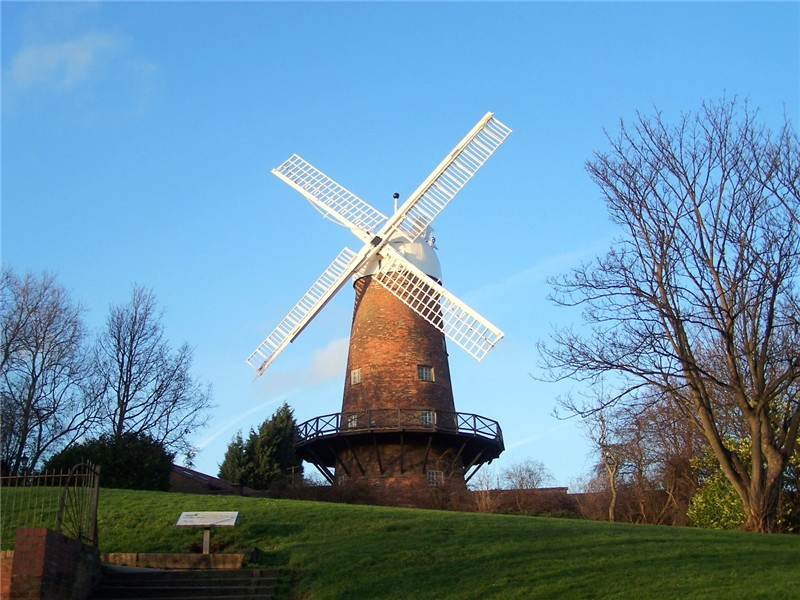
\includegraphics[width=8cm]{images/greens_windmill} 
	\caption{Windm�hle, in der Green f�r lange Zeit gearbeitet hat} 
	\label{fig:abb1} 
	\end{figure} 